\documentclass[12pt]{article}

\usepackage{amsmath}
\usepackage{amssymb}
\usepackage[dvips]{graphicx}
%\usepackage{lscape}
\usepackage{eepic}
\usepackage{color}
\usepackage{wasysym} % \female \male
\usepackage[landscape,pdftex]{geometry}
\usepackage{fancyhdr}
\usepackage{hyperref}

\definecolor{cantelope}{rgb}{1.0,0.8,0.4}
\hypersetup{
    colorlinks, urlcolor={cantelope}
}
\hypersetup{pdfpagemode=UseNone} % don't show bookmarks on initial view

\DeclareOption{bigsym}{\DeclareSymbolFont{largesymbols}{OMX}{psycm}{m}{n}}
\ProcessOptions

\setlength{\oddsidemargin}{-0.75in}
\setlength{\evensidemargin}{-0.75in}
\setlength{\topmargin}{-1in}
\setlength{\textheight}{7.75in}
\setlength{\textwidth}{10.5in}
\setlength{\footskip}{0in}
\setlength{\parindent}{0pt}
\setlength{\rightskip}{0pt plus 1fil} % makes ragged right

\renewcommand{\familydefault}{phv} % helvetica

% following: color
\definecolor{mybgcolor}{rgb}{0,0,0.3125}
\definecolor{myyellow}{rgb}{1,1,0.4}
\definecolor{myblue}{rgb}{0.4,0.8,1}
\definecolor{mypink}{rgb}{1,0.4,1}
\definecolor{mywhite}{rgb}{1,1,1}

% following: B/W
%\definecolor{mybgcolor}{rgb}{1,1,1}
%\definecolor{myyellow}{rgb}{0,0,0}
%\definecolor{myblue}{rgb}{0,0,0}
%\definecolor{mypink}{rgb}{0,0,0}
%\definecolor{mywhite}{rgb}{0,0,0}

% header/footer layout
\pagestyle{fancy}
\lhead{} \chead{} \rhead{}
\lfoot{} \cfoot{} \rfoot{\color{myyellow} \thepage}
\renewcommand{\headrulewidth}{0pt}
\renewcommand{\footrulewidth}{0pt}

% font sizes
\newcommand{\superlarge}{\fontsize{60}{60} \selectfont}
\newcommand{\titlesize}{\fontsize{40}{50} \selectfont}
\newcommand{\headsize}{\fontsize{35}{35} \selectfont}
\newcommand{\textsize}{\fontsize{30}{35} \selectfont}
\newcommand{\smallsize}{\fontsize{25}{30} \selectfont}
\newcommand{\smallersize}{\fontsize{20}{25} \selectfont}
\newcommand{\smallestsize}{\fontsize{18}{22} \selectfont}
\newcommand{\lod}{\text{LOD}}
\newcommand{\rss}{\text{RSS}}
\newcommand{\var}{\text{var}}
\newcommand{\M}{\text{M}}
%\renewcommand{\log}{\text{log}}
%\renewcommand{\max}{\text{max}}



\pagecolor{mybgcolor}
\color{mywhite}

\begin{document}
\thispagestyle{empty}

\begin{center}
\titlesize \color{myyellow}


\vspace*{15mm}

QTL mapping 2: Special topics

\color{mypink}
\rule{10in}{1mm}
%\vspace{-10mm}

\vspace{5mm}

\textsize \color{myblue}
Karl Broman
\vspace{5mm}

\color{mywhite}
{\smallsize Biostatistics and Medical Informatics

University of Wisconsin -- Madison
\vspace{20mm}


\href{http://kbroman.org}{\tt kbroman.org} \\[3pt]
\href{https://github.com/kbroman}{\tt github.com/kbroman} \\
\href{https://twitter.com/kwbroman}{\tt @kwbroman}
}

\end{center}


\newpage

\headsize \color{myyellow}
\hfill \begin{minipage}{5.75in}
\centering
Selection bias
\end{minipage}

\vspace{15mm}

\color{mywhite} \smallsize

\hspace*{0.5in}
\begin{minipage}[t]{4.1in}
\vspace*{5mm}

\sloppy
\smallestsize
\begin{itemize}
\setlength{\rightskip}{0pt plus 1fil} % makes ragged right
\item The estimated effect of a QTL will vary somewhat from its true
effect.
\item Only when the estimated effect is large will the QTL be
detected.
\item Among those experiments in which the QTL is detected, the estimated
QTL effect will be, on average, larger than its true effect.
\item This is {\color{mypink} selection bias}.
\item Selection bias is largest in QTLs with small or moderate effects.
\item The true effects of QTLs that we identify are likely smaller
than was observed.
\end{itemize}
\end{minipage}
\hfill
\begin{minipage}[t]{5.3in}
\vspace*{0mm}

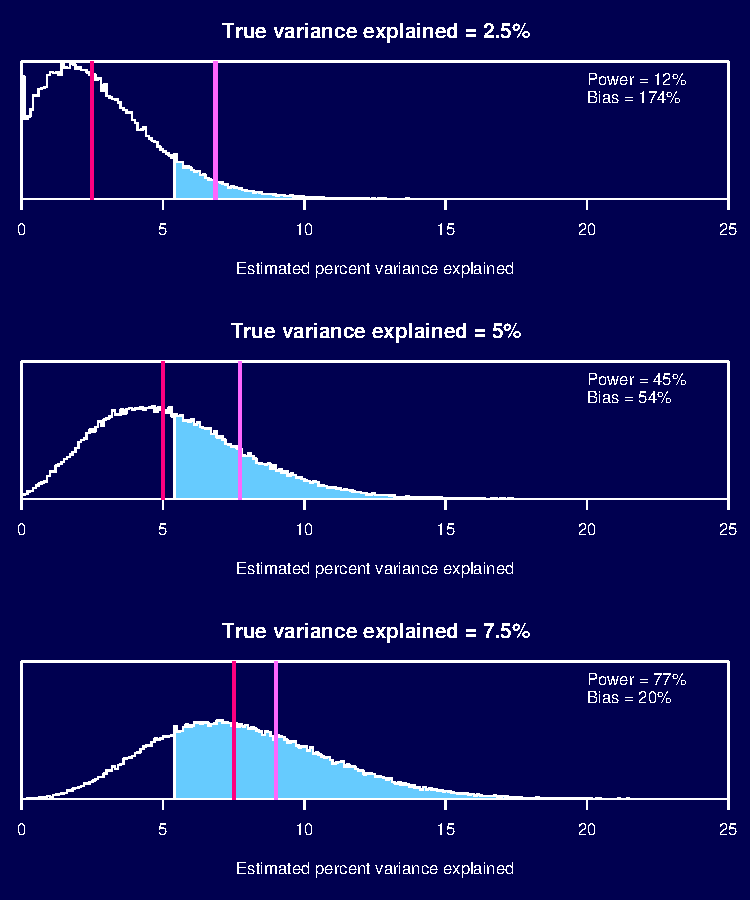
\includegraphics{Figs/selbias.pdf}
\end{minipage}

\newpage

\headsize \color{myyellow}
\hfill \begin{minipage}{5.75in}
\centering
Implications
\end{minipage}

\smallsize \color{mywhite}

\vspace{25mm}

\hfill
\begin{minipage}{10in}
\begin{itemize}
\setlength{\itemsep}{24pt}
\item Estimated \% variance explained by identified QTLs

\item Repeating an experiment

\item Congenics (aka near isogenic lines)

\item Marker-assisted selection
\end{itemize}
\end{minipage}



\newpage

\headsize \color{myyellow}
\hfill \begin{minipage}{5.75in}
\centering
Non-normal traits
\end{minipage}


\vspace{25mm}

\color{mywhite} \smallersize
\hfill \begin{minipage}{10in}
\begin{itemize}
\setlength{\rightskip}{0pt plus 1fil} % makes ragged right
\itemsep18pt
\item Standard interval mapping assumes normally distributed residual
variation.  (Thus the phenotype distribution is a mixture of normals.)
\item {\color{mypink} In reality}: we see dichotomous traits,
counts, skewed distributions, outliers, and all sorts of odd things.
\item Interval mapping, with LOD thresholds derived from permutation
tests, generally performs just fine anyway.
\item Alternatives to consider:
\begin{itemize}
\smallersize
\setlength{\rightskip}{0pt plus 1fil} % makes ragged right
    \item Nonparametric approaches {\color{myblue} (Kruglyak \& Lander 1995)}
    \item Transformations {\color{myblue} (\emph{e.g.}, log, square root, normal quantiles)}
    \item Specially-tailored models  {\color{myblue} (\emph{e.g.}, a generalized linear
    model, the Cox proportional hazard model, and the two-part model
    in Broman 2003)}
\end{itemize}
\end{itemize} \end{minipage}




\newpage

\headsize \color{myyellow}
\hfill \begin{minipage}{5.75in}
\centering
Haley-Knott regression
\end{minipage}

\vspace{3cm}

\color{mywhite} \smallsize

\hspace*{0.5in}
A quick approximation to Interval Mapping.

\smallersize

\begin{eqnarray*}
\mathsf{E(y_i | q_i)} & = & \mathsf{ \mu_q } \\[24pt]
\mathsf{E(y_i | M_i)} & = & \mathsf{E[ \ E(y_i|q_i) \ | M_i]}
 =  \mathsf{\textstyle{\sum_j \Pr(q=j|M_i) \mu_j}} \\[12pt]
& = & \mathsf{\textstyle{\sum_j p_{ij} \mu_j}}
\end{eqnarray*}

\vspace{1cm}

\hfill \begin{minipage}{10in}
\setlength{\rightskip}{0pt plus 1fil} % makes ragged right
{\color{mypink} Regress $\mathsf{y}$ on $\mathsf{p_i}$}, pretending the residual
variation is normally distributed (with constant variance).
\end{minipage}

\begin{eqnarray*}
\mathsf{\lod} & = & \mathsf{\frac{n}{2} \log_{10} \left( \frac{\rss_0}{\rss_1} \right)}
\end{eqnarray*}

\newpage

\headsize \color{myyellow}
\hfill \begin{minipage}{5.75in}
\centering
The normal mixtures
\end{minipage}

\vspace{15mm}

\hspace*{0.5in}
\begin{minipage}[t]{4.6in}
\vspace*{10mm}

\color{mywhite} \smallersize
\setlength{\unitlength}{1.0in}
\begin{center}
\begin{picture}(4.5,1)
% lines
\Thicklines
\put(0.25,0.5){\line(1,0){4}}
\put(0.25,0.35){\line(0,1){0.3}}
\put(1.65,0.35){\line(0,1){0.3}}
\put(4.25,0.35){\line(0,1){0.3}}

% text
\put(0.25,0.1){\makebox(0,0){$\mathsf{M_1}$}}
\put(4.25,0.1){\makebox(0,0){$\mathsf{M_2}$}}
\put(1.65,0.1){\makebox(0,0){$\mathsf{Q}$}}
\put(0.95,0.8){\makebox(0,0){7 cM}}
\put(2.95,0.8){\makebox(0,0){13 cM}}
\end{picture} \end{center}
\vspace{5mm}

\begin{itemize}
\setlength{\rightskip}{0pt plus 1fil} % makes ragged right
\item Two markers separated by 20 cM, with the QTL closer to the left marker.
\item The figure at right shows the distributions of the phenotype
conditional on the genotypes at the two markers.
\item The dashed curves correspond to the components of the mixtures.
\end{itemize}

\end{minipage}
\hfill
\begin{minipage}[t]{4.6in}
\vspace*{0mm}

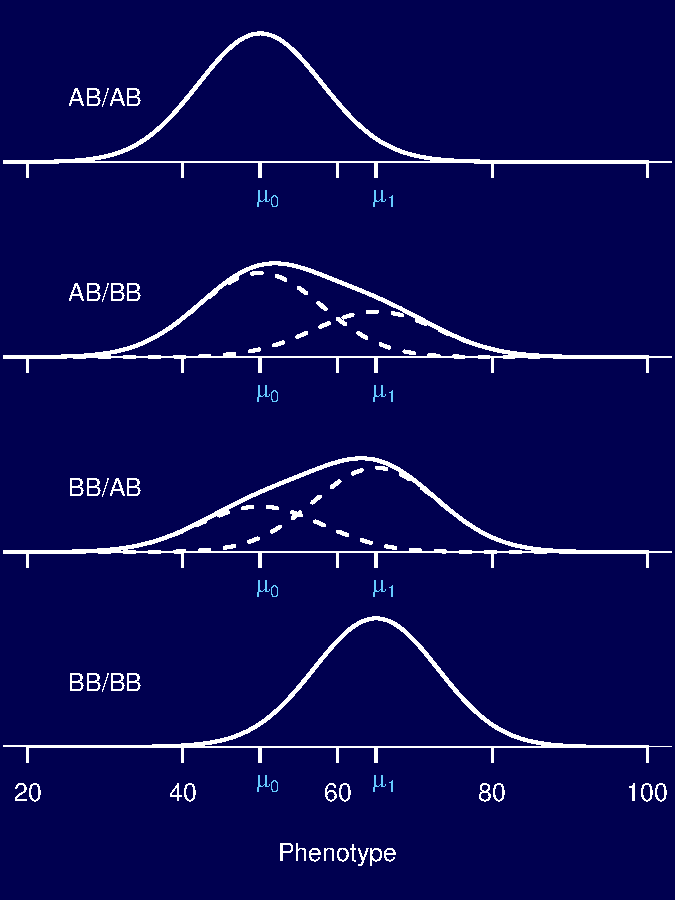
\includegraphics{Figs/mixtures.pdf}
\end{minipage}




\newpage

\headsize \color{myyellow}
\hfill \begin{minipage}{5.75in}
\centering
Haley-Knott results
\end{minipage}

\vfill

\centerline{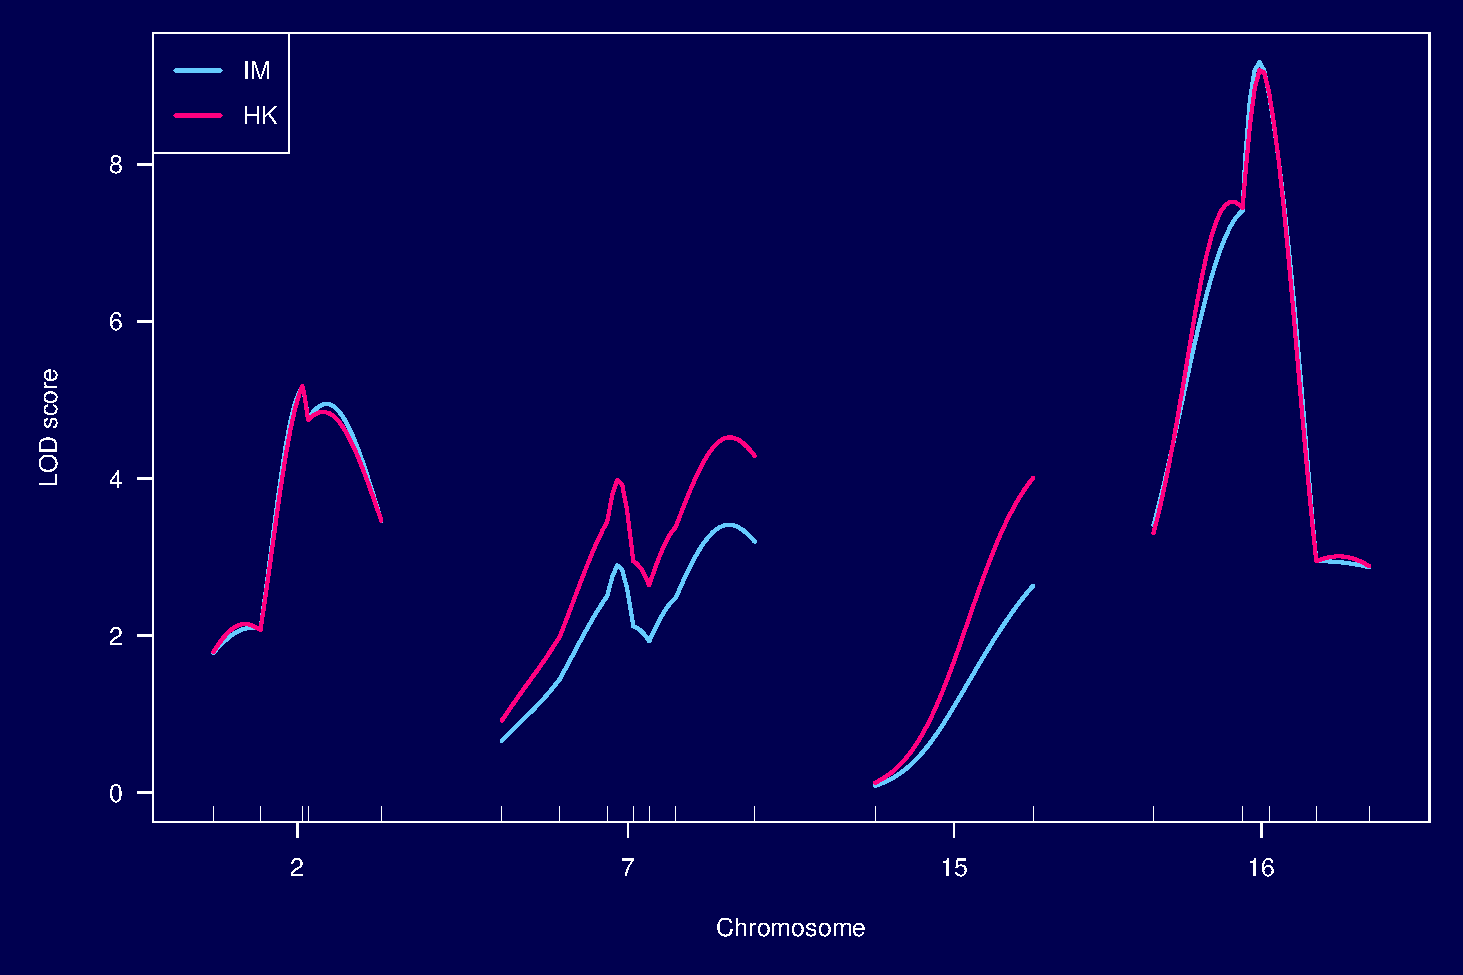
\includegraphics{Figs/hk_lod.pdf}}



\newpage

\headsize \color{myyellow}
\hfill \begin{minipage}{5.75in}
\centering
H-K with selective genotyping
\end{minipage}

\vfill

\centerline{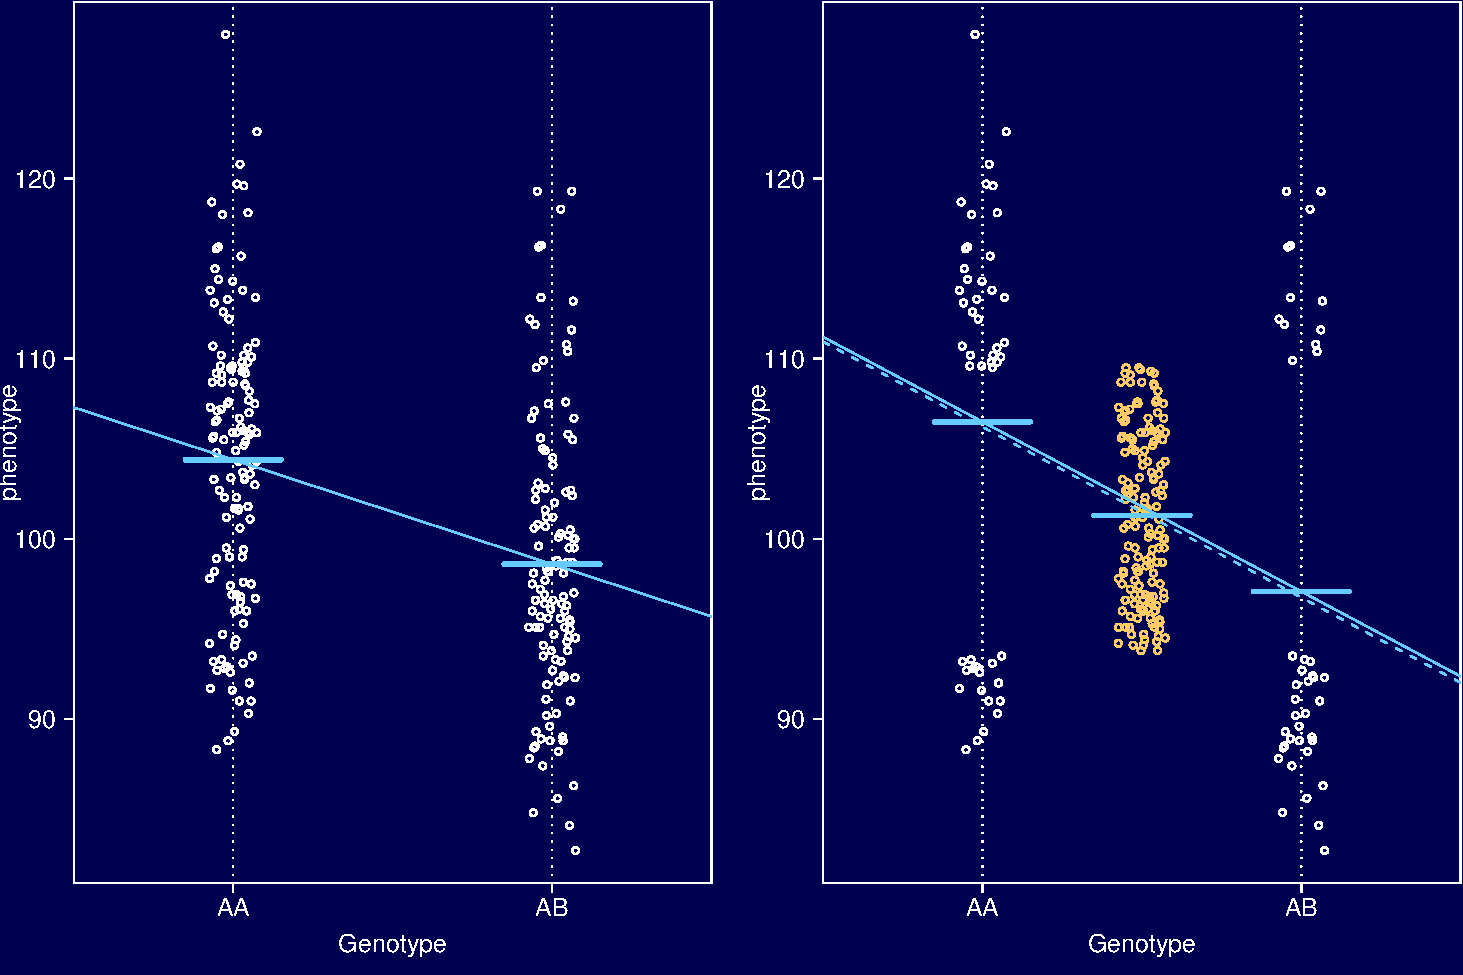
\includegraphics{Figs/hk_selgeno.pdf}}





\newpage

\headsize \color{myyellow}
\hfill \begin{minipage}{5.75in}
\centering
Multiple imputation
\end{minipage}

\vfill

\centerline{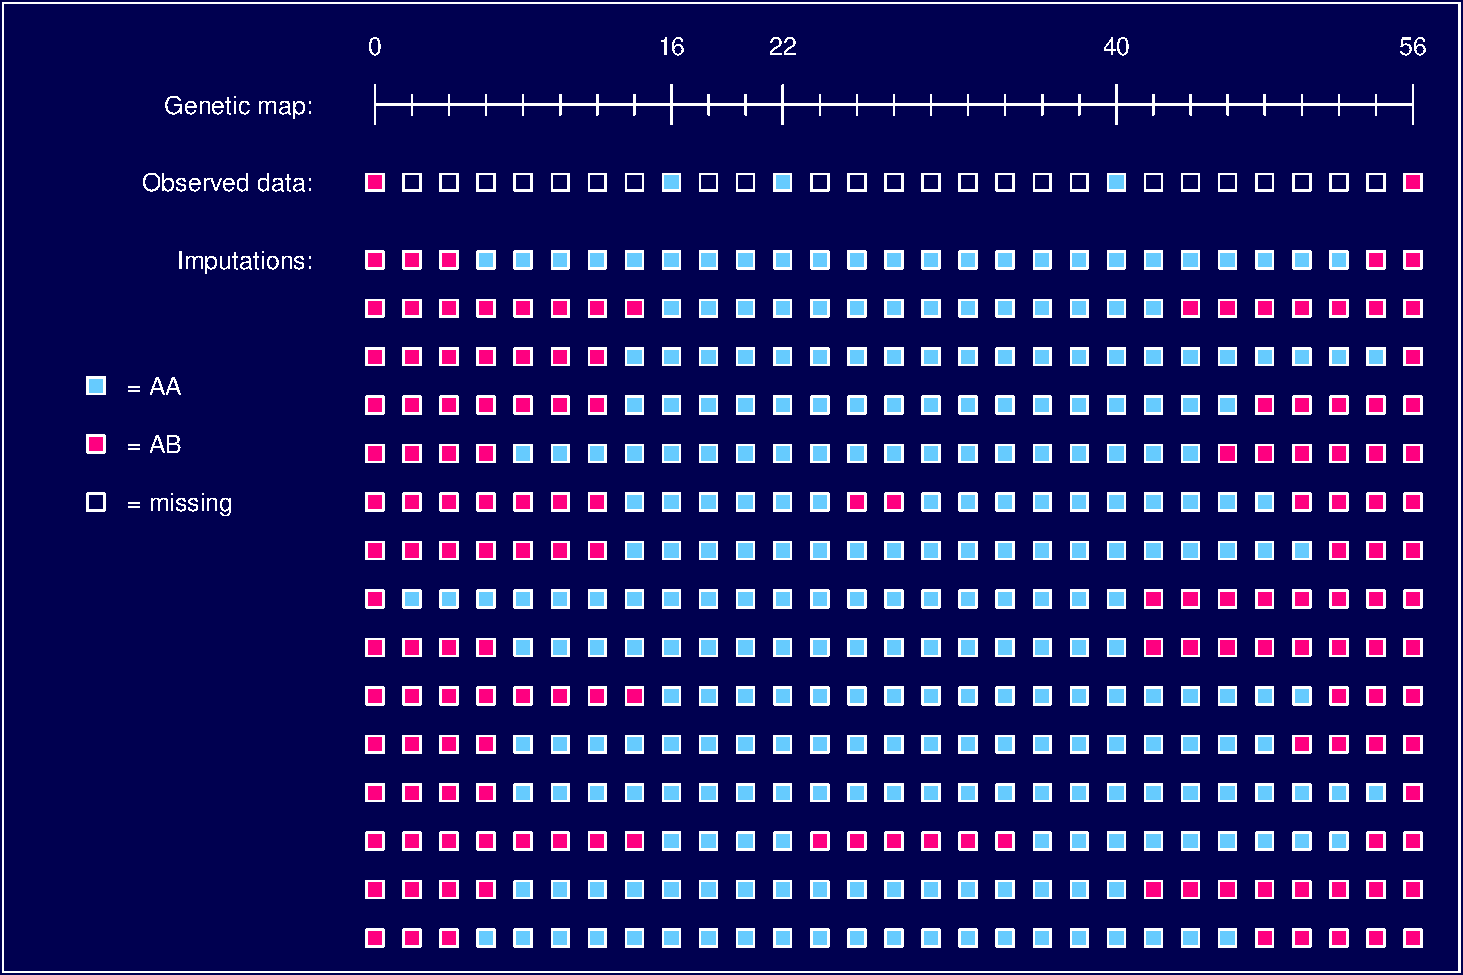
\includegraphics{Figs/imp.pdf}}


\newpage

\headsize \color{myyellow}
\hfill \begin{minipage}{5.75in}
\centering
Multiple imputations
\end{minipage}

\vfill

\centerline{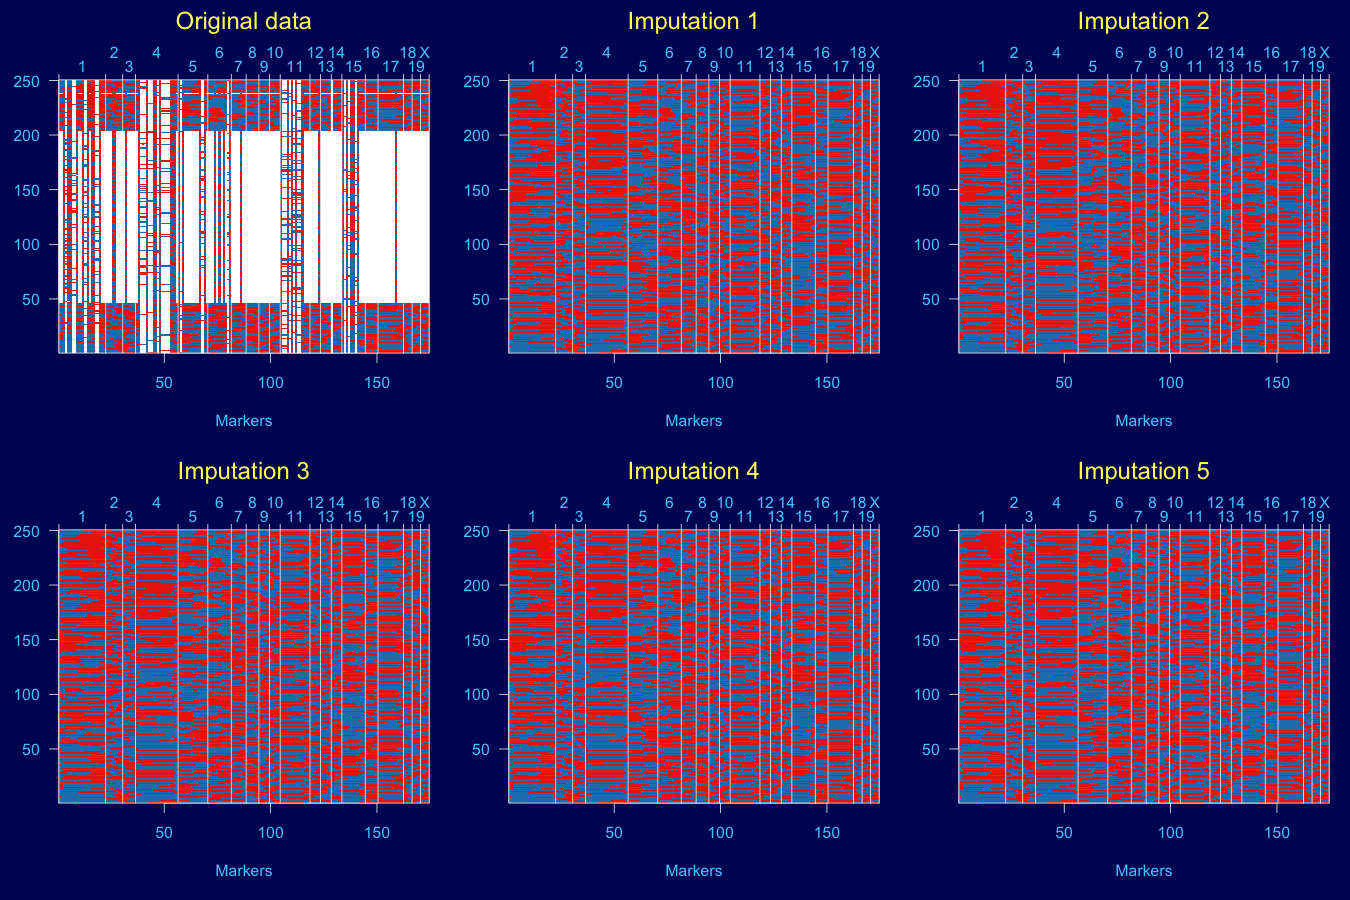
\includegraphics[height=6.5in]{Figs/multiimp.png}}



\newpage

\headsize \color{myyellow}
\hfill \begin{minipage}{5.75in}
\centering
Imputation LOD curves
\end{minipage}

\vfill

\centerline{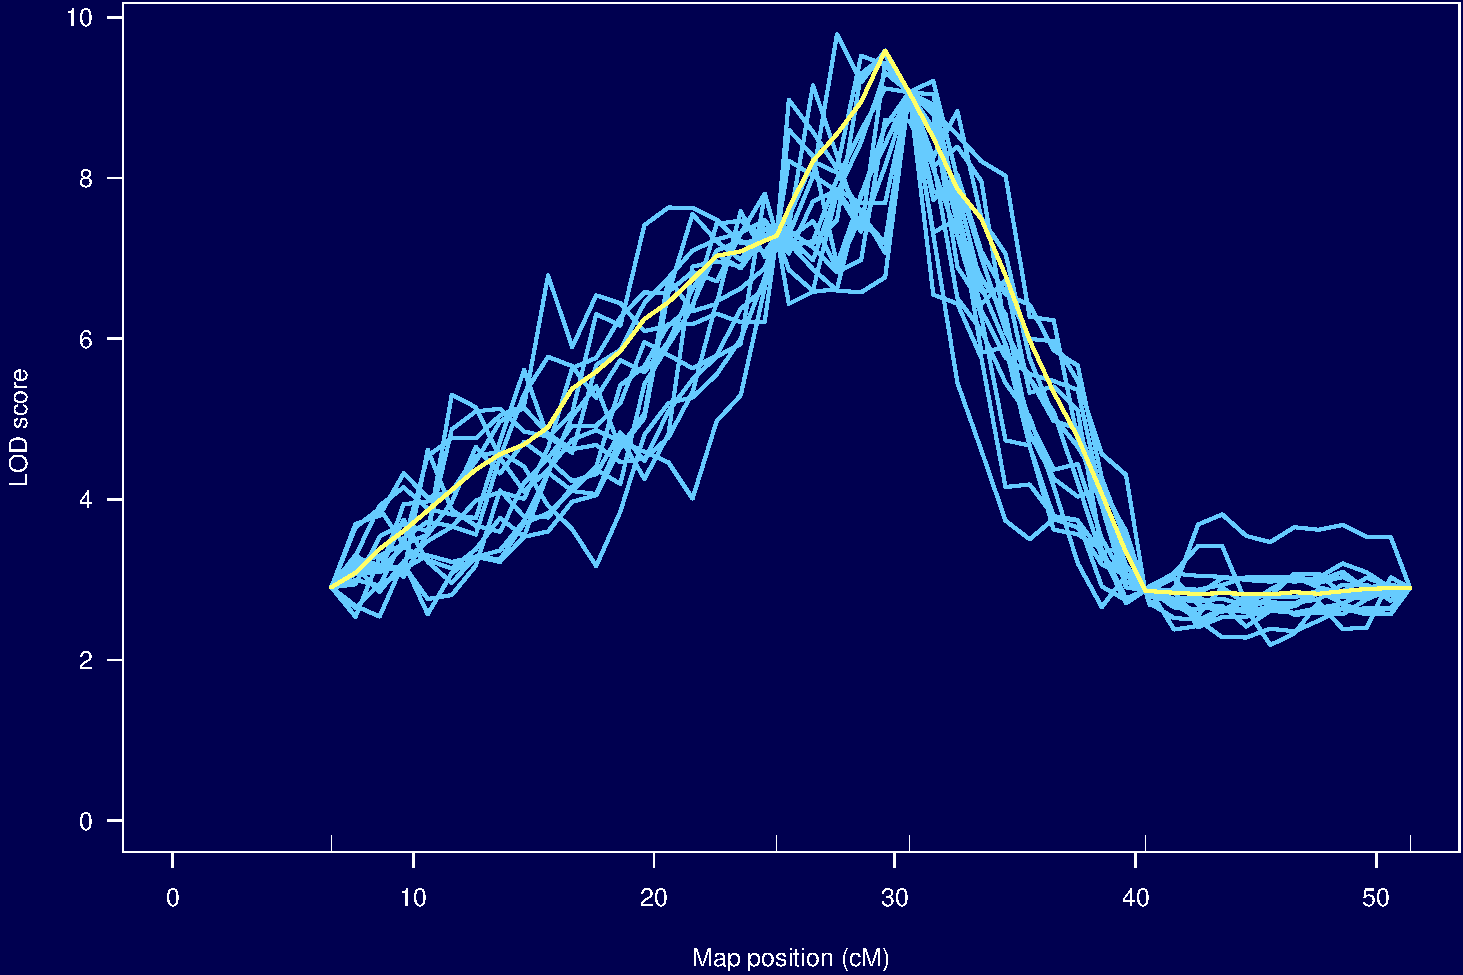
\includegraphics{Figs/imp_lod.pdf}}



\newpage

\headsize \color{myyellow}
\hfill \begin{minipage}{5.75in}
\centering
Summary comparison
\end{minipage}


\vspace{25mm}

\begin{center}
\color{mywhite}
\smallersize

\renewcommand\arraystretch{2}
\begin{tabular}{cccccc}
\hline
Approach & Speed & Extensibility & Stability & Missing data &
Parallelization \\
\hline
HK & ++ & + & + & -- & ++ \\
EM & + & $-$ & $-$ & + & $-$ \\
%% Extended HK & ++ & $-$ & + & + & $-$ \\
Imputation & $-$ & + & + & + & + \\
%Extended Haley-Knott & + & - & ++ & ++ \\
\hline
\end{tabular}
\end{center}


\newpage

\headsize \color{myyellow}
\hfill \begin{minipage}{5.75in}
\centering
Covariates
\end{minipage}

\vspace{15mm}

\color{mywhite} \smallsize

\hspace*{0.5in}
\begin{minipage}[t]{4.1in}
\vspace*{25mm}

\sloppy
\smallestsize
\begin{itemize}
\setlength{\rightskip}{0pt plus 1fil} % makes ragged right
\item {\color{mypink} Examples} : treatment, sex, litter, lab, age.
\item Control residual variation.
\item Avoid confounding.
\item Look for QTL $\times$ covariate interactions
\end{itemize}
\end{minipage}
\hfill
\begin{minipage}[t]{5.3in}
\vspace*{0mm}

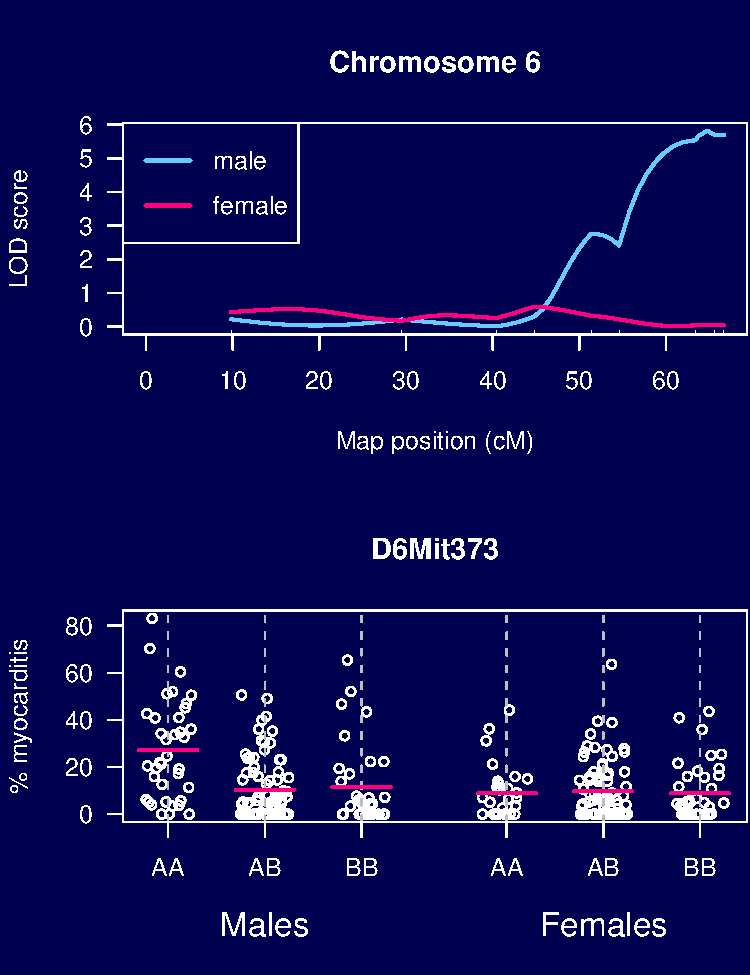
\includegraphics{Figs/covar.pdf}
\end{minipage}




\newpage

\headsize \color{myyellow}
\hfill X chr in backcross

\vfill

\centerline{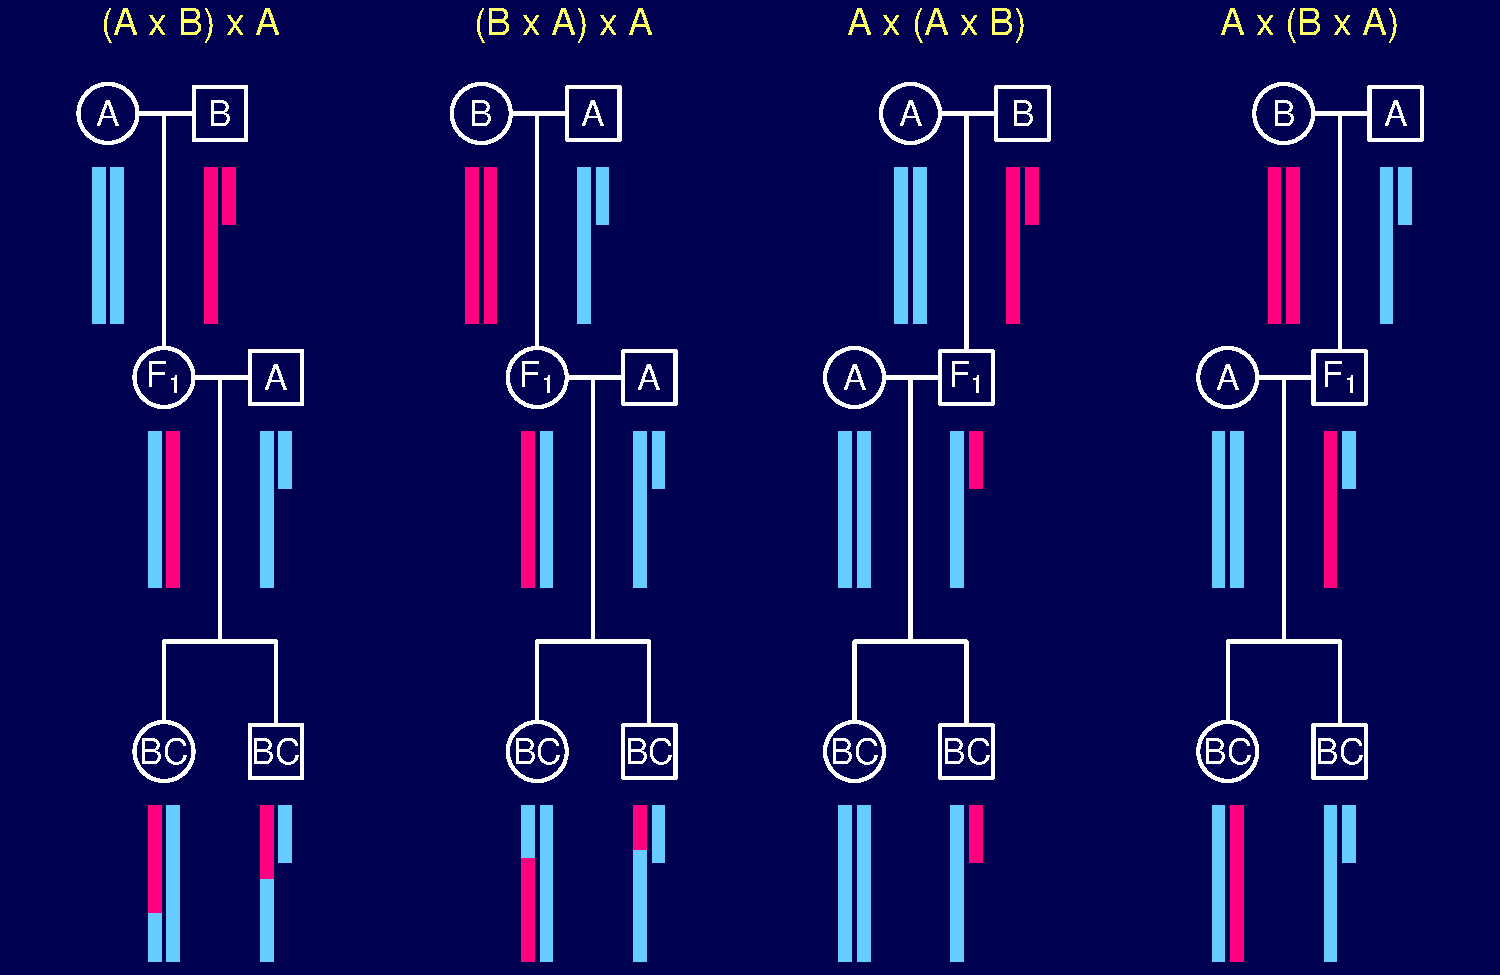
\includegraphics[]{Figs/xchr_bc.pdf}}


\newpage

\headsize \color{myyellow}
\hfill X chr in intercross

\vfill

\centerline{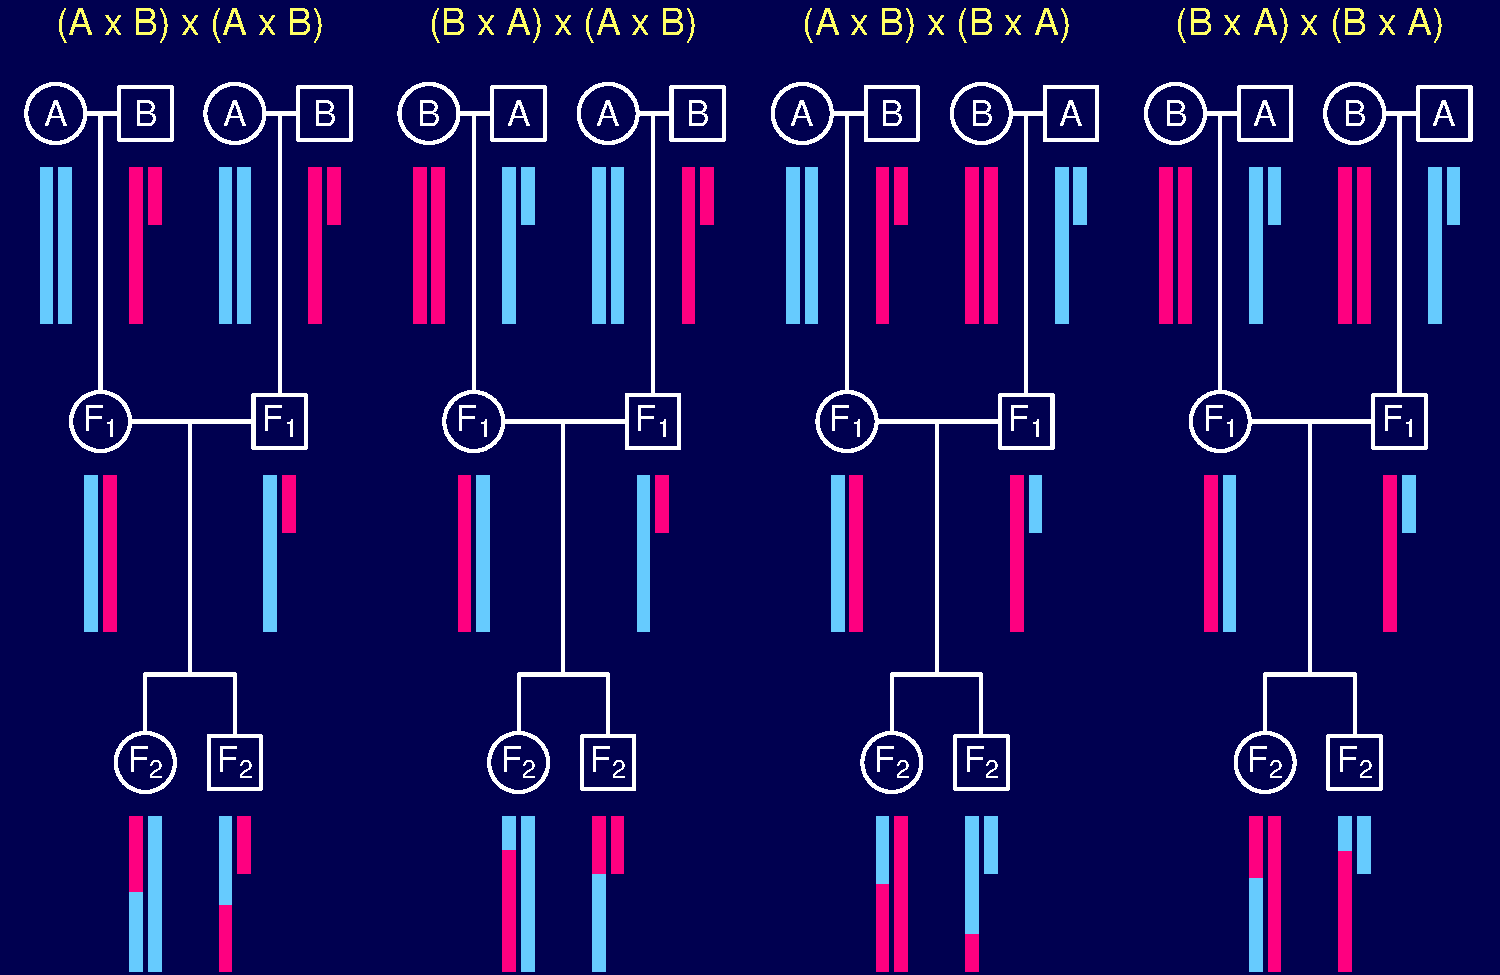
\includegraphics[]{Figs/xchr_f2.pdf}}




\newpage

\headsize \color{myyellow}
\hfill Example

\vspace{3cm}

\color{mywhite} \textsize

Intercross: both dir, both sexes

\vspace{20mm}

\color{myblue} \smallsize

\hspace*{1in} \begin{tabular}{cccccccccccc}
{\textsize \female} & forward & \hspace{1cm} & AA & or & AB \\[18pt]
{\textsize \female} & reverse &              &    &    & AB & or & BB \\[18pt]
{\textsize   \male} & forward &            &    &    &    &    &    & AY & or & BY \\[18pt]
{\textsize   \male} & reverse &              &    &    &    &    &    & AY & or & BY
\end{tabular}





\newpage

\headsize \color{myyellow}
\hfill Principles

\vspace{3cm}

\color{mywhite} \smallsize

\hfill \begin{minipage}[t]{9.5in}
\begin{itemize}
\itemsep24pt
\item Sex- or cross-direction-difference in the phenotype shouldn't
  lead to spurious linkage on the X chromosome
\item Simple as possible
\item Null nested within alternative
\end{itemize} \end{minipage}


\newpage

\headsize \color{myyellow}
\hfill Approach

\smallersize \color{mywhite}
\vspace{2cm}

\begin{center}
\setlength{\tabcolsep}{12pt}
\renewcommand{\arraystretch}{1.5}
\noindent \begin{tabular}{cccccc} \hline
{\color{myblue} Cross} & {\color{myblue} Direction} & {\color{myblue} Sexes} & {\color{myblue} Contrasts} & {\color{myblue} H$_{\text{0}}$} & {\color{myblue} df} \\ \hline
BC & & both& AA:AB:AY:BY & $\female$:$\male$ & 2
  \\
BC & & $\female$ & AA:AB & grand mean & 1 \\
BC & & $\male$ & AY:BY & grand mean & 1 \\ \hline
F$_{\text{2}}$ & both & both & AA:ABf:ABr:BB:AY:BY & $\female_{f}$:$\female_{r}$:$\male$ & 3 \\
F$_{\text{2}}$ & both & $\female$ & AA:ABf:ABr:BB & $\female_{f}$:$\female_{r}$ & 2
  \\
F$_{\text{2}}$ & both & $\male$ & AY:BY & grand mean & 1 \\
F$_{\text{2}}$ & one  & both & AA:AB:AY:BY & $\female$:$\male$ & 2 \\
F$_{\text{2}}$ & one  & $\female$ & AA:AB & grand mean & 1 \\
F$_{\text{2}}$ & one  & $\male$ & AY:BY & grand mean & 1 \\
\hline
\end{tabular} \end{center}



\newpage

\headsize \color{myyellow}
\hfill Chromosome-specific thresholds

\vspace{2cm}

\color{mywhite} \smallsize

Let {\color{myblue} $\alpha_i$} = false positive rate for chromosome $i$.

\bigskip

We need {\color{myblue} $1 - \alpha = \prod (1 - \alpha_i)$}

\bigskip \bigskip \bigskip

For example,  {\color{myblue} $\alpha_1 = \alpha$ {\color{mywhite} and} $\alpha_j = 0$
  for $j \ne 1$}

\bigskip \bigskip \bigskip

The usual method: {\color{mypink} constant LOD threshold} \\
\hspace*{3in} {\color{myblue} (i.e., constant power)}

\bigskip \bigskip \bigskip

{\color{myyellow} My approach: \hspace{1cm} $\alpha_i \propto L_i$}
\hspace{1cm} where $L_i$ = length of chr $i$

\bigskip \bigskip

\hspace*{1.5in} {\color{myblue} Similar and more convenient:  $\alpha_i = (1-\alpha)^{L_i/L}$}




\newpage

\headsize \color{myyellow}
\hfill \begin{minipage}{5.75in}
\centering
Data diagnostics
\end{minipage}

\vspace{3cm}

\color{mywhite} \smallsize

\hfill \begin{minipage}[t]{9.5in}
\begin{itemize}
\itemsep18pt
\item Plot phenotypes
\item Look for sample duplicates
\item Look for excessive missing data
\item Investigate segregation distortion
\item Verify genetic maps/marker positions
\item Look for genotyping errors
\item Look at counts of crossovers
\end{itemize} \end{minipage}




\end{document}
